








%\begin{frame}{Limitations de \texttt{keybert}}
%	\danger{} manque de diversification des résultats + (non-)grammaticalité\\
%	\begin{figure}[!ht]
%		\centering
%		\includegraphics[width=110mm,scale=0.5]{pic/termes\_keybert\_autres.png}
%		\caption{Répartition des 15 termes les plus pertinents dans le corpus \og{}Autres\fg{} selon \texttt{keybert}.}
%		\label{fig:enter-label}
%	\end{figure}
%\end{frame}

%\begin{frame}{Phrases-clés \textit{hapax} partagés dans les deux corpus selon \texttt{keybert}}
%	Les seuls termes partagés avec le corpus Charcot : 
%	%\begin{itemize}
%	%\item articulations de [\textit{sic}] épaule
%	%\item paralysie faciale périphérique
%	%\end{itemize}
%	\begin{figure}[!ht]
%		\centering
%		\includegraphics[width=90mm,scale=0.5]{pic/termes\_partages\_keybert.png}
%		\caption{Répartition des termes les plus pertinents dans les deux corpus selon \texttt{keybert}.}
%		\label{fig:enter-label}
%	\end{figure}
%\end{frame}


%\begin{frame}{Termes partagés extraits avec \texttt{keyphrase-vectorizers}}
%    \begin{figure}[!ht]
	%        \centering
	%        \includegraphics[width=85mm,scale=0.5]{pic/visualisation_termes_dupliques.png}
	%        \caption{Les termes communs aux deux corpus selon \texttt{keyphrase-vectorizers}.}
	%        \label{fig:enter-label}
	%    \end{figure}
%\end{frame}

%\begin{frame}{Termes partagés | \texttt{keyphrase-vectorizers}}
%    \begin{figure}[!ht]
	%        \centering
	%        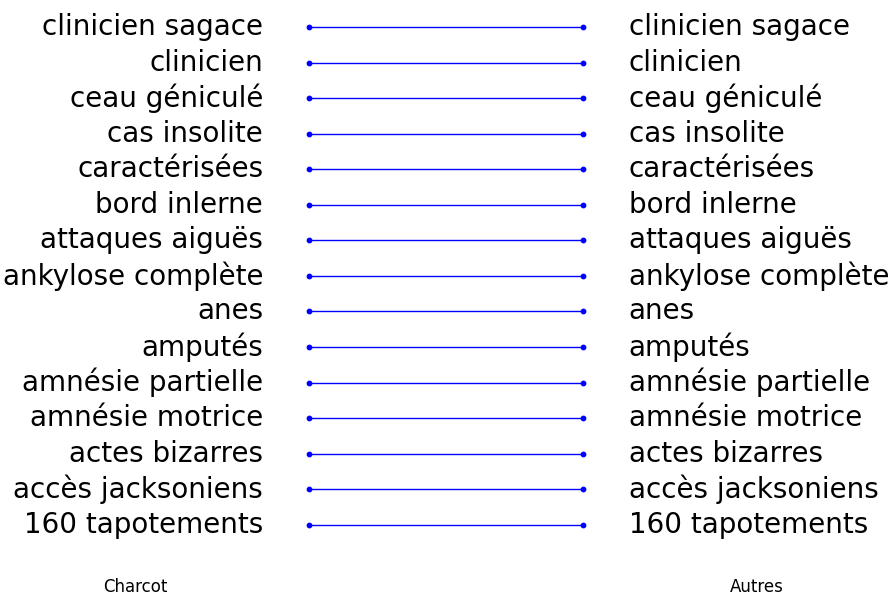
\includegraphics[width=100mm,scale=0.5]{pic/termes_partages_liens.png}
	%        \caption{Les termes communs (fréq. = 1) aux deux corpus selon \texttt{keyphrase-vectorizers}.}
	%        \label{fig:enter-label}
	%    \end{figure}
%\end{frame}




\begin{frame}{Les termes partagés les plus fréquents | \texttt{keyphrase-vectorizers}}
	\begin{figure}[!ht]
		\centering
		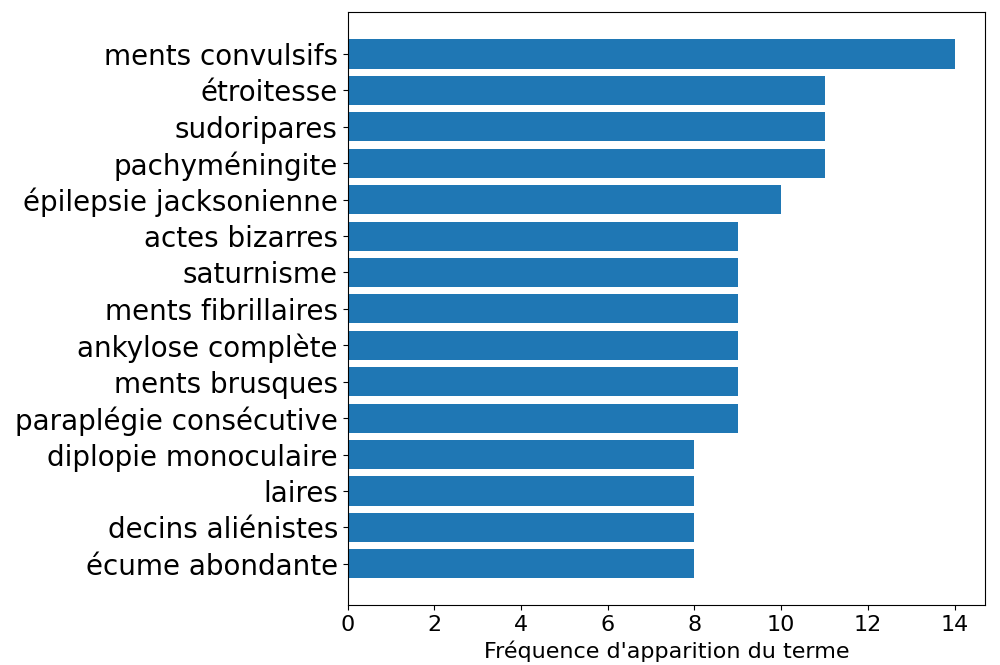
\includegraphics[width=100mm,scale=0.5]{pic/termes_partages.png}
		\caption{Les 15 termes les plus fréquents dans les deux corpus selon \texttt{keyphrase-vectorizers}.}
		\label{fig:enter-label}
	\end{figure}
\end{frame}



\begin{frame}{Les termes les plus impactants}
	\begin{itemize}
		\item  \textbf{tics convulsifs} (\textit{PatternRank}), \textbf{hypnose} (moyenne)
		\item \textit{PatternRank} valorise systématiquement les termes
		\item pas de consensus entre les métriques
%		\begin{itemize}
%			\item l'écart le plus petit entre eux : \textit{hypnose}
%		\end{itemize}
	\end{itemize}
	\begin{figure}[h]
		\centering
		\includegraphics[width=\linewidth]{pic/termes_viz.png}
		\caption{Scores de pertinences pour chaque terme de référence, corpus \og{}Autres\fg{}.}
		\label{fig:ling_out_TAL}
	\end{figure}
\end{frame}



%\begin{frame}{Accès à la plateforme technologique \textsc{MeSU}}
%\begin{itemize}
%\item expériences réalisées sur la plateforme \href{https://sacado.sorbonne-universite.fr/}{\textsc{MeSU}} de Sorbonne Université
%\end{itemize}
%\bigskip
%
%Les données et les scripts utilisés dans le cadre de cette étude sont disponibles sur le \href{https://github.com/ljpetkovic/JE\_IA\_HN\_030524}{dépôt GitHub}.
%\end{frame}

%\begin{frame}{Analyse comparative des approches employées}
%	\begin{itemize}
%		\item \textit{PatternRank} valorise systématiquement les termes
%		\item pas de consensus entre les métriques
%		\begin{itemize}
%			\item l'écart le plus petit entre eux : \textit{hypnose}
%		\end{itemize}
%	\end{itemize}
%	\begin{figure}[h]
%		\includegraphics[width=\linewidth]{pic/termes_viz.png}
%		\caption{Visualisation des scores de pertinences pour chaque terme de référence.}
%		\label{fig:ling_out_TAL}
%	\end{figure}
%\end{frame}